\documentclass{beamer}

\usepackage{hyperref}
\usepackage{pgfplots}
\usepackage{tikz}
\usetikzlibrary{intersections}

\usetheme{Warsaw}

\title[Optimising UAR Sampling]{Faster by Design: Optimising UAR Sampling for Grammar Inference}
\author[Antriksh Dhand]{\textbf{Antriksh Dhand}\\{\small Supervised by Dr Rahul Gopinath}}
\date{February 9th, 2024}

\institute[USYD]
{
	School of Computer Science\\
	The University of Sydney
}

\AtBeginSection[]
{
  \begin{frame}
    \frametitle{Table of Contents}
    \tableofcontents[currentsection]
  \end{frame}
}

\begin{document}

%%%%%%%%%%%%%%%%%%%%%%%%%
	\begin{frame}
	\titlepage
	\end{frame}
%%%%%%%%%%%%%%%%%%%%%%%%%

	\section*{Outline}

%%%%%%%%%%%%%%%%%%%%%%%%%
	\begin{frame}{Table of Contents}
	\tableofcontents
	\end{frame}
%%%%%%%%%%%%%%%%%%%%%%%%%

	\section{Background}

	\subsection{Introduction to GI}
%%%%%%%%%%%%%%%%%%%%%%%%%
	\begin{frame}{A brief introduction}

		Imagine you're in a new country and all the signs are in a foreign language. The act of slowly picking up words and patterns from these signs is analagous to grammar inference.
	
	\end{frame}
%%%%%%%%%%%%%%%%%%%%%%%%%

%%%%%%%%%%%%%%%%%%%%%%%%%
	\begin{frame}{A brief introduction}

		\begin{definition}[Grammar Inference]
			The process of automatically learning or inferring the \alert{underlying rules and structure} of a formal grammar from a set of observed strings.	
		\end{definition}
	
	\end{frame}
%%%%%%%%%%%%%%%%%%%%%%%%%

%%%%%%%%%%%%%%%%%%%%%%%%%
\begin{frame}[fragile]{What is a formal grammar?}
	Using a formal grammar, we can define a (very) small subset of all the possible strings in the English language.
	\begin{exampleblock}{English v2.0}
		\begin{verbatim}
		<sentence> ::= <noun_phrase> <verb>
		<noun_phrase> ::= <article> <noun>
		<article> ::= "a" | "the"
		<noun> ::= "horse" | "dog" | "hamster"
		<verb> ::= "stands" | "walks" | "jumps"
		\end{verbatim}
		For example: \texttt{"A horse stands"} is a valid string in our language.
	\end{exampleblock}
\end{frame}
%%%%%%%%%%%%%%%%%%%%%%%%%

%%%%%%%%%%%%%%%%%%%%%%%%%
	\begin{frame}{Applications of GI}
		\framesubtitle{Sentiment analysis}

		\includegraphics[width=0.5\textwidth]{img/chatgpt1.png}%
		\includegraphics[width=0.5\textwidth]{img/chatgpt2.png}

		Grammar inference is used in sentiment analysis to help extract the grammatical structures or patterns associated with positive or negative sentiments in reviews.
	\end{frame}
%%%%%%%%%%%%%%%%%%%%%%%%%

% %%%%%%%%%%%%%%%%%%%%%%%%%
% 	\begin{frame}{Applications of GI}
% 		\framesubtitle{Sentiment analysis}

% 		By identifying these grammatical structures associated with sentiments, a sentiment analysis model can be trained to recognise and categorise reviews accurately.
% 		\vspace{7pt}
% 		\begin{examples}
% 			\begin{itemize}
% 				\item Positive reviews often contain ``highly recommend", ``excellent service", etc.
% 				\item Negative reviewers may use shorter sentences and negations such as ``didn't enjoy"
% 			\end{itemize}
% 		\end{examples}

% 	\end{frame}
% %%%%%%%%%%%%%%%%%%%%%%%%%

% %%%%%%%%%%%%%%%%%%%%%%%%%
% 	\begin{frame}[fragile]{Applications of GI}
% 		\framesubtitle{Sentiment analysis}

% 		The output of running grammar inference for sentiment analysis is a formal grammar, like the one we saw above:

% 		\begin{verbatim}
% 			<review> ::= <positive> | <negative>
% 			<positive> ::= "The" <subject> "is" <positiveAdj>
% 			<subject> ::= "product" | "service" | "experience"
% 			<positiveAdj> ::= "excellent" | "amazing" | "quality"
% 			...
% 		\end{verbatim}

% 		Example production: \texttt{The product is amazing.}
% 	\end{frame}
% %%%%%%%%%%%%%%%%%%%%%%%%%

%%%%%%%%%%%%%%%%%%%%%%%%%
	\begin{frame}{Grammar inference: a broad field}
	
		\centering
		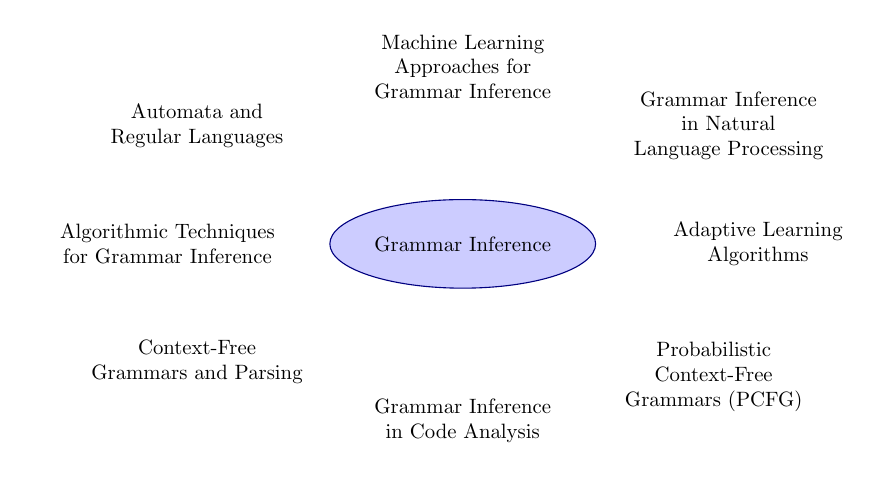
\begin{tikzpicture}[scale=0.75, transform shape]
			% Draw cloud shape
			\draw[fill=blue!20,draw=blue!50!black] (0,0) ellipse (2.25 and 0.75);
			\node[align=center] at (0,0) {Grammar Inference};
			
			% Draw phrases around the cloud
			\node[text width=3.5cm, align=center] at (-4.5,2) {Automata and Regular Languages};
			\node[text width=5cm, align=center] at (-4.5,-2) {Context-Free\\Grammars and Parsing};
			\node[text width=3.5cm, align=center] at (4.25,-2.25) {Probabilistic Context-Free Grammars (PCFG)};
			\node[text width=4.5cm, align=center] at (-5,0) {\alert{Algorithmic Techniques\\for Grammar Inference}};
			\node[text width=4.5cm, align=center] at (4.5,2) {Grammar Inference\\in Natural\\Language Processing};
			\node[text width=3.5cm, align=center] at (0,-3) {Grammar Inference in Code Analysis};
			\node[text width=3.5cm, align=center] at (0,3) {Machine Learning Approaches for Grammar Inference};
			\node[text width=3cm, align=center] at (5,0) {Adaptive Learning Algorithms};
		\end{tikzpicture}
	\end{frame}
%%%%%%%%%%%%%%%%%%%%%%%%%

	\subsection{Comparison of GI algorithms}
	
%%%%%%%%%%%%%%%%%%%%%%%%%
	\begin{frame}{Choosing the best GI algorithm}

		There are many grammar inference algorithms out there:
		\begin{itemize}
			\item Angluin L* + extensions
			\item TTT algorithm
			\item ARVADA
			\item GLADE
			\item ...
		\end{itemize}

		What measure do we use to say that one grammar inference algorithm is better than another?

	\end{frame}
%%%%%%%%%%%%%%%%%%%%%%%%%

%%%%%%%%%%%%%%%%%%%%%%%%%
	\begin{frame}{Quantifying ``better"}
		Let the original grammar (the one we are trying to infer) be denoted $G$. Let the output of the grammar inference algorithm be $G'$.

		\begin{fact}
			A grammar inference algorithm is ``good" if $G'$ is \alert{similar} to $G$.
		\end{fact}
	\end{frame}
%%%%%%%%%%%%%%%%%%%%%%%%%

%%%%%%%%%%%%%%%%%%%%%%%%%
\begin{frame}{Quantifying ``better"}
	We measure similarity using two measures:
	\begin{definition}[Precision]
		If we run a generating fuzzer on $G'$, how close is the output to running a parser on $G$?

		% Practically, this means that if you take the inferred grammar $G'$ and generate strings from it using a fuzzer, how many of these strings will be valid according to the original grammar $G$? A high precision value indicates that the inferred grammar produces strings that closely match the expected output of the original grammar.

	\end{definition}
	\begin{definition}[Recall]
		If we run a generating fuzzer on G, how close is the output to running a parser on G'?

		% This implies that if you take the original grammar $G$, generate strings from it using a fuzzer, and then run a parser on $G'$, how many of these strings will be successfully parsed by the inferred grammar? A high recall value indicates that the inferred grammar captures the patterns and structures present in the original grammar.
	\end{definition}
	Note: the generation must be \alert{uniform at random.}\\i.e. when sampling a string $s$ from a grammar, $P(s) = c, c \in \mathbb{R}$.
\end{frame}
%%%%%%%%%%%%%%%%%%%%%%%%%

%%%%%%%%%%%%%%%%%%%%%%%%%
	\begin{frame}[c]{Quantifying ``better"}
		We combine Precision and Recall using the F1 score:
		\begin{definition}
			$$\text{F1 score} = \frac{2 \times \text{Precision} \times \text{Recall}}{\text{Precision} + \text{Recall}}$$
		\end{definition}
		\vspace{30pt}
		Comparing effectiveness of grammar inference algorithms is then equivalent to comparing F1 scores.
	\end{frame}
%%%%%%%%%%%%%%%%%%%%%%%%%

	\subsection{Project scope} % Motivation

%%%%%%%%%%%%%%%%%%%%%%%%%
\begin{frame}{Broad project goal}
	\begin{alertblock}{}
		Set up a toolchain to compare grammar inference algorithms.
	\end{alertblock}
\end{frame}
%%%%%%%%%%%%%%%%%%%%%%%%%

%%%%%%%%%%%%%%%%%%%%%%%%%
	\begin{frame}{A pathway to comparison}
		\begin{columns}
			\begin{column}{0.3\textwidth}
				The pathway to comparison is extensive and involves multiple stages. We've designed a phased approach to address the complexity of the project. 
			\end{column}
			\begin{column}{0.7\textwidth}
				\centering
				\includegraphics[width=0.95\textheight]{img/pyramid.png}
			\end{column}
		\end{columns}
	\end{frame}
%%%%%%%%%%%%%%%%%%%%%%%%%

%%%%%%%%%%%%%%%%%%%%%%%%%
	\begin{frame}{Phase 1: Problem statement}
		\begin{alertblock}{Challenge}
			Many current algorithms for UAR sampling are written in Python which is a slower, interpreted language.
			% \item Rely on string operations and lots of memory allocations.
		\end{alertblock}
		\begin{itemize}
			\item Would ChatGPT be as successful if each query took 5 minutes to run?
			% \begin{itemize}
			% 	\item e.g. the formal grammar specification for the C programming language is several pages long
			% \end{itemize}
			\item In practice, efficiency is key.
			\item To pave the way for future advancements, we must utilise a high-performance language and optimise the code for efficiency.
		\end{itemize}

	\end{frame}
%%%%%%%%%%%%%%%%%%%%%%%%%

%%%%%%%%%%%%%%%%%%%%%%%%%
	\begin{frame}{Phase 1: Goals}
		\begin{enumerate}
			\item Build more efficient tools, structures, and functions to work with grammars.
			\item Implement UAR sampling using this foundation.
		\end{enumerate}

		% Limited time constraints necessitate a strategic approach to achieve our project goal effectively. We've designed a phased approach to tackle the complexities of the task at hand.

		% In the initial phase, our focus is on laying down the foundational groundwork for grammar representation in C and implementing Uniform At Random (UAR) sampling. Within a tight 2-month timeframe, we aim to establish the infrastructure required to handle grammars efficiently.

		% However, considering the constraints, we've refined our scope to prioritize fundamental techniques like UAR sampling in C. This ensures that we make significant progress within the allotted time while setting the stage for more advanced implementations in subsequent phases.
		
	\end{frame}
%%%%%%%%%%%%%%%%%%%%%%%%%

	\section{Methodology}

	\subsection{Optimising grammar representation}

%%%%%%%%%%%%%%%%%%%%%%%%%
\begin{frame}{Why C}
			
	\begin{itemize}
		\item C is a compiled language, leading to \alert{faster execution times} compared to interpreted languages like Python.
		\item C offers \alert{manual memory management} which allows us control over using dynamic or static allocation, enhancing efficiency and performance. 
	\end{itemize}

\end{frame}
%%%%%%%%%%%%%%%%%%%%%%%%%

%%%%%%%%%%%%%%%%%%%%%%%%%
	\begin{frame}{Developing foundations}
			
		\begin{block}{}
			Set up a robust and optimised method of storing a grammar in C.
		\end{block}
		\vspace{10pt}

		Instead of using strings in our representation, we map each token in the grammar to an 8-bit number.
		\begin{itemize}
			\item Non-terminals are assigned 8-bit keys starting from \texttt{0x80}
			\item Terminals are assigned 8-bit keys starting from \texttt{0x00}
		\end{itemize}
		\vspace{10pt}
		This allows us to:
		\begin{itemize}
			\item Check if a token is non-terminal in $O(1)$ time (MSB)
			\item Greatly improve the space complexity of our algorithms
		\end{itemize}		

	\end{frame}
%%%%%%%%%%%%%%%%%%%%%%%%%

%%%%%%%%%%%%%%%%%%%%%%%%%
\begin{frame}[fragile]{Developing foundations}
				
	\begin{verbatim}
		<expression> ::= <term> "+" <term>
		<term> ::= <factor> "*" <factor>
		<factor> ::= "0" | "1" | "2" | ... | "9"
	\end{verbatim}
	The above grammar would be converted to:
	\begin{verbatim}
		0x80 ::= 0x81 0x00 0x81
		0x81 ::= 0x82 0x01 0x82 
		0x82 ::= 0x02 | 0x03 | 0x04 | ... | 0x0B 
	\end{verbatim}

\end{frame}
%%%%%%%%%%%%%%%%%%%%%%%%%

%%%%%%%%%%%%%%%%%%%%%%%%%
	\begin{frame}[fragile]{Developing foundations}
				
		We also store tokens in our representation in the order they appear in the grammar i.e. grammars are stored as such:
		\begin{verbatim}
			GRAMMAR = [<NT-struct for 0x80>, <NT-struct for 0x81>,
			<NT-struct for 0x82>, ...]
		\end{verbatim}

		\begin{itemize}
			\item This allows us $O(1)$ time index lookup of each non-terminal in the grammar (4 least significant bits)
		\end{itemize}

	\end{frame}
%%%%%%%%%%%%%%%%%%%%%%%%%

	\subsection{JSON-to-C converter}

%%%%%%%%%%%%%%%%%%%%%%%%%
	\begin{frame}[fragile]{Allowing ``plug-and-play" functionality} 
		\begin{block}{}
			Develop a program to convert existing grammar to C representation.
		\end{block}
		\vspace{10pt}
		As most researchers use JSON to represent their grammars, we developed a JSON-to-C converter to jumpstart the development process for users.
		

	\end{frame}
%%%%%%%%%%%%%%%%%%%%%%%%%

%%%%%%%%%%%%%%%%%%%%%%%%%
	\begin{frame}{Allowing ``plug-and-play" functionality} 
	    \begin{tikzpicture}[remember picture,overlay]
			\node[at=(current page.center), yshift=-20pt] {
				\includegraphics[width=0.9\paperwidth]{img/jsontoc.png}
			};
		\end{tikzpicture}
	\end{frame}
%%%%%%%%%%%%%%%%%%%%%%%%%

	\subsection{Implementing UAR sampling}

%%%%%%%%%%%%%%%%%%%%%%%%%
	\begin{frame}{UAR sampling implementation}

		\begin{itemize}
			\item Fuzzers' string sampling may lack uniformity due to their reliance on grammar structure. 
			\item Our approach generates \alert{all potential strings} from the grammar.
			\item We then employ random sampling from the exhaustive set of strings, ensuring uniform distribution.
			\item This method guarantees robust and reliable sampling, overcoming the limitations of conventional fuzzers.
		\end{itemize}
	\end{frame}
%%%%%%%%%%%%%%%%%%%%%%%%%

%%%%%%%%%%%%%%%%%%%%%%%%%
	\begin{frame}{UAR sampling implementation}
		\begin{block}{}
			Use efficient data structures to implement sampling algorithm.
		\end{block}
		We implemented custom hash tables in C to memoize the grammar's structure.
		\begin{itemize}
			\item \texttt{KeyNode} and \texttt{RuleNode} objects were created in C to represent Keys and Rules in the grammar.
			\item The memoization process involves recursively traversing the grammar rules and storing these objects in hash tables.
			\item By storing previously computed results, redundant computations are avoided, optimising the sampling process.
		\end{itemize}
	\end{frame}
%%%%%%%%%%%%%%%%%%%%%%%%%

%%%%%%%%%%%%%%%%%%%%%%%%%
\begin{frame}[fragile]{UAR sampling implementation}
	We utilised \alert{Jenkins' one-at-a-time} hash function to try and obtain a uniform spread of keys in the hash tables and minimise collisions.
	\begin{small}
		\begin{verbatim}
			uint32_t hash = 0;

			for (size_t i = 0; i < 8; ++i) {
			    hash += key & 1;
			    hash += (hash << 10);
			    hash ^= (hash >> 6);
			    key >>= 1;
			}

			hash += (hash << 3);
			hash ^= (hash >> 11);
			hash += (hash << 15);
		\end{verbatim}
	\end{small}
\end{frame}
%%%%%%%%%%%%%%%%%%%%%%%%%

	\section{Results}

%%%%%%%%%%%%%%%%%%%%%%%%%
	\begin{frame}{Performance improvements}

		\begin{center}
			Our C implementation of a basic fuzzer was up to\\
			\vspace{10pt} % Adjust the space as needed
			{\Huge % Adjust the size as needed
			23x faster} \\ % Your big number here 
			\vspace{10pt} % Adjust the space as needed
			than its Python counterpart.
		\end{center}
		
	\end{frame}
%%%%%%%%%%%%%%%%%%%%%%%%%

%%%%%%%%%%%%%%%%%%%%%%%%%
\begin{frame}{Performance improvements}
	\centering
	\includegraphics[height=0.85\textheight]{img/fuzzergraph.png}
\end{frame}
%%%%%%%%%%%%%%%%%%%%%%%%%

%%%%%%%%%%%%%%%%%%%%%%%%%
\begin{frame}{Performance improvements}

	\begin{center}
		Our C implementation of the UAR sampling algorithm ran up to\\
		\vspace{10pt} % Adjust the space as needed
		{\Huge % Adjust the size as needed
		14x faster} \\ % Your big number here 
		\vspace{10pt} % Adjust the space as needed
		than its Python counterpart.	
	\end{center}
	
\end{frame}
%%%%%%%%%%%%%%%%%%%%%%%%%

%%%%%%%%%%%%%%%%%%%%%%%%%
\begin{frame}{Performance improvements}
	\centering
	\includegraphics[height=0.85\textheight]{img/uargraph.png}
\end{frame}
%%%%%%%%%%%%%%%%%%%%%%%%%

%%%%%%%%%%%%%%%%%%%%%%%%%
	\begin{frame}{Contribution to the field}
		\begin{itemize}
			\item Our findings not only substantiate the foundational work we have done in optimising our grammar structure but also provide a valuable and accessible asset to the programming community.
			\item The transparent documentation ensures accessibility and encourages collaborative exploration in the field of grammar inference.
		\end{itemize}
		
	\end{frame}
%%%%%%%%%%%%%%%%%%%%%%%%%

	\section{Conclusion}

%%%%%%%%%%%%%%%%%%%%%%%%%
	\begin{frame}{Future work}
		\centering
		\includegraphics[height=0.8\textheight]{img/pyramid.png}
	\end{frame}
%%%%%%%%%%%%%%%%%%%%%%%%%

%%%%%%%%%%%%%%%%%%%%%%%%%
\begin{frame}{Resources}
	\begin{columns}
		\begin{column}{0.7\textwidth}
			The code produced as a result of this research project is now a well-documented open-source C library and can be accessed at \textcolor{cyan}{\href{https://github.com/antrikshdhand/gfuzztools}{github.com/antrikshdhand/gfuzztools}}.
		\end{column}
		\begin{column}{0.3\textwidth}
			\centering
			\includegraphics[width=\textwidth]{img/gfuzztools.png}
		\end{column}
	\end{columns}
\end{frame}
%%%%%%%%%%%%%%%%%%%%%%%%%

%%%%%%%%%%%%%%%%%%%%%%%%%
\begin{frame}{Acknowledgements}
	I am sincerely grateful for the time and effort invested by \textcolor{cyan}{
	\href{https://www.sydney.edu.au/engineering/about/our-people/academic-staff/rahul-gopinath.html}{Dr. Rahul Gopinath}} in sharing his expertise, providing valuable suggestions, and serving as an inspiring mentor throughout this project. 
\end{frame}
%%%%%%%%%%%%%%%%%%%%%%%%%

%%%%%%%%%%%%%%%%%%%%%%%%%
	\begin{frame}
		\centering
		\vspace{10pt}
		\Huge \textbf{Thank You}
		\vspace{30pt}
		\large
		\begin{block}{Contact information}
			\begin{itemize}
				\item Email: \textcolor{cyan}{\href{mailto:adha5655@uni.sydney.edu.au}{adha5655@uni.sydney.edu.au}}
				\item GitHub: \textcolor{cyan}{\href{https://github.com/antrikshdhand}{github.com/antrikshdhand}}
				\item LinkedIn: \textcolor{cyan}{\href{https://www.linkedin.com/in/antrikshdhand}{linkedin.com/in/antrikshdhand}}
			\end{itemize}
	\end{block}
	\end{frame}
%%%%%%%%%%%%%%%%%%%%%%%%%

%%%%%%%%%%%%%%%%%%%%%%%%%
\begin{frame}{References and further reading}
	\begin{thebibliography}{Dijkstra, 1982}
	\bibitem[Gopinath, 2021]{Gopinath2021}
		R.~Gopinath.
		\newblock Uniform Random Sampling of Strings from Context-Free Grammar
		\newblock \textcolor{cyan}{\href{https://rahul.gopinath.org/post/2021/07/27/random-sampling-from-context-free-grammar/}{rahul.gopinath.org}}, 2021.

	\bibitem[Dijkstra, 1982]{Dijkstra1982}
		C.~Higuera.
		\newblock Grammatical Inference: Learning Automata and Grammars
		\newblock Cambridge University Press, 2010.

	\bibitem[Angluin, 1987]{Angluin1987}
		D.~Angluin.
		\newblock Learning Regular Sets from Queries and Counterexamples
		\newblock {\em Information and Computation}, 2(75):87--106, 1982.
	\end{thebibliography}
\end{frame}	
%%%%%%%%%%%%%%%%%%%%%%%%%

\end{document}
